% Copy the relevant figure environments into the manuscript.
% Adjust the graphicspath or filenames for your manuscript folder.

\begin{figure}[t]
\centering
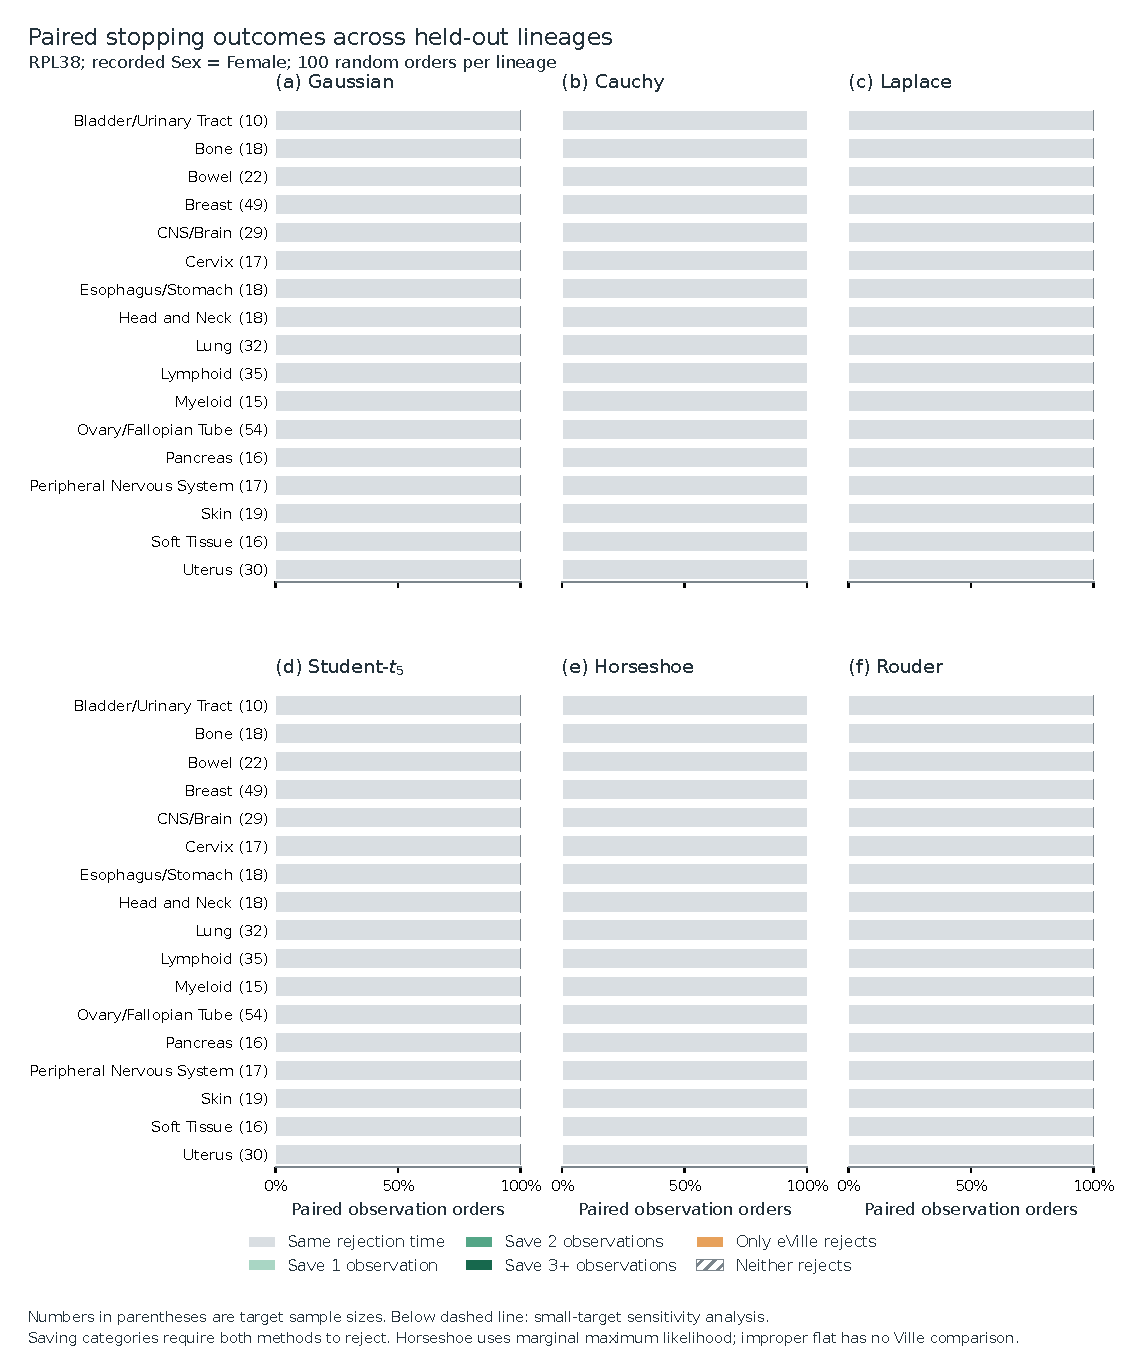
\includegraphics[width=\textwidth]{results/figures/paired_savings_all_lineages.pdf}
\caption{Paired stopping outcomes for the RPL38 leave-one-lineage-out experiment. Each bar summarises 100 random orders of the same held-out sample, shared across priors and calibration methods; the original ModelID order is excluded. Among orders for which both methods reject, colours show equal stopping times or the number of observations saved by eVille. Orders with eVille-only rejection and orders with neither rejection are separate categories. The 17 main lineages have at least ten observations; seven smaller lineages are shown below the dashed separator as sensitivity results. Numbers in parentheses are target sample sizes. The improper flat comparator has no ordinary Ville comparison and is therefore absent. Gaussian, Cauchy, Laplace and Student-$t_5$ fits use full-family maximum likelihood; Horseshoe* uses the explicitly stated median/IQR exception. These fractions describe ordering sensitivity conditional on the observed data, not repeated-sample power.}
\label{fig:rpl38-paired}
\end{figure}

\begin{figure}[t]
\centering
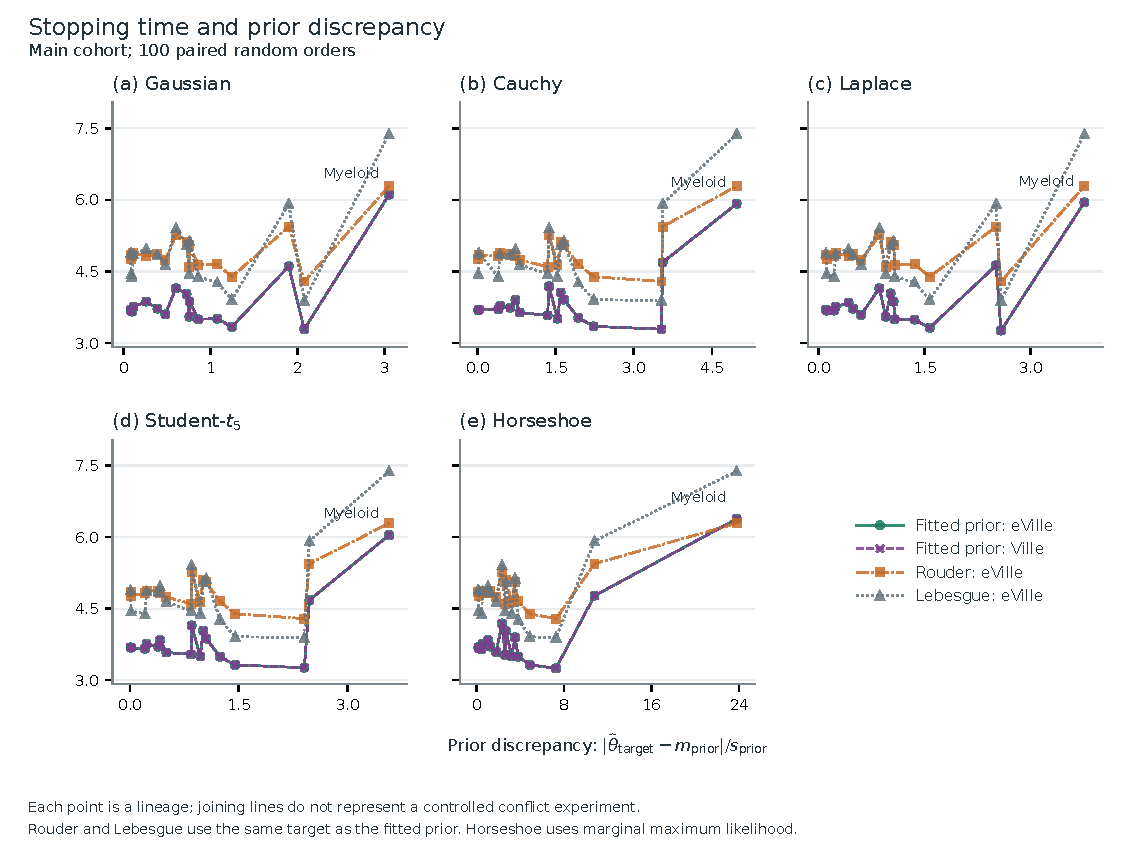
\includegraphics[width=\textwidth]{results/figures/conflict_and_flat_baseline.pdf}
\caption{Descriptive source--target displacement and stopping times relative to the improper flat baseline, for the 17 main lineages. The horizontal coordinate is $|\widehat\theta_g-\widehat m_{-g}|/\widehat s_{-g}$, where $\widehat m_{-g}$ and $\widehat s_{-g}$ are the full-family prior location and scale fitted to source-lineage estimates. The scale is not generally a standard deviation, and this coordinate is not a calibrated conflict statistic. Vertical coordinates are mean restricted stopping times minus the flat-prior eVille mean, using the same 100 orders. Zero denotes equal mean restricted observation use. Paired eVille and Ville points share the same lineage and prior. Myeloid is highlighted. This cross-lineage comparison varies sample size, target effect and fitted prior; it does not establish a monotone conflict--power relation or a limiting convergence result. Horseshoe* denotes the quantile-fit exception.}
\label{fig:rpl38-conflict}
\end{figure}

\begin{figure}[t]
\centering
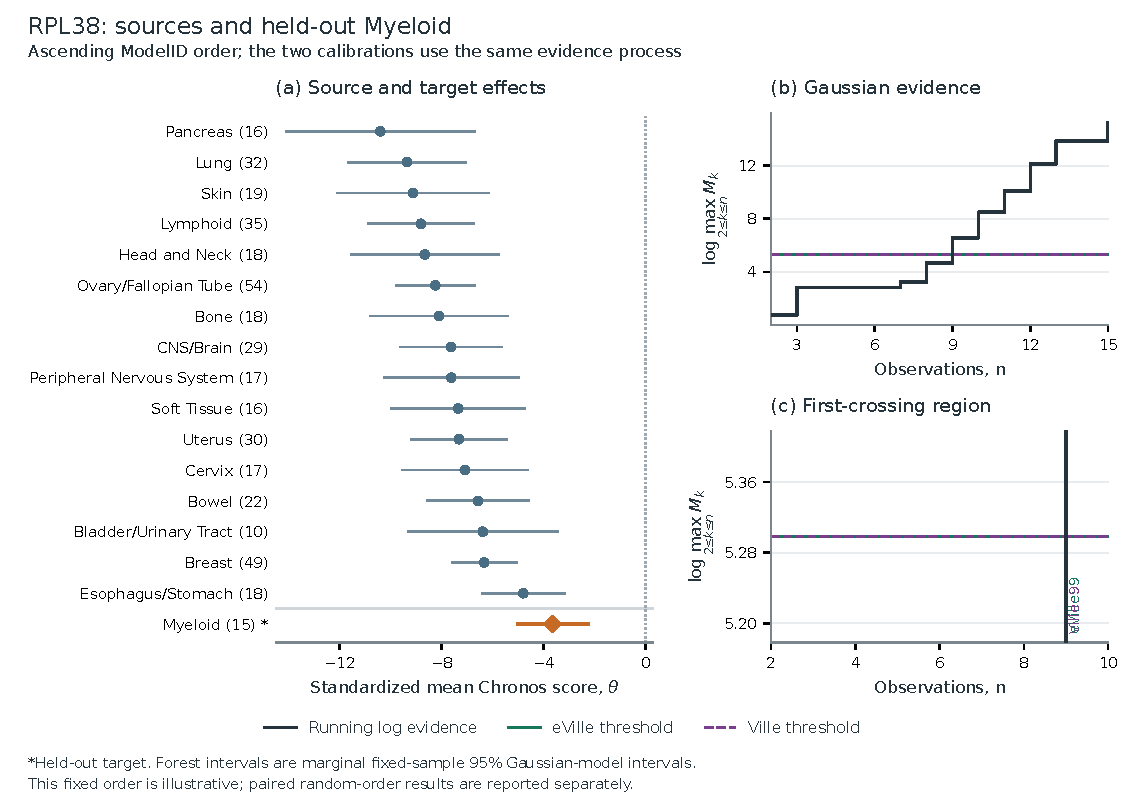
\includegraphics[width=\textwidth]{results/figures/example_forest_and_evidence.pdf}
\caption{Illustrative held-out Myeloid analysis. The forest plot shows source-lineage standardized mean Chronos estimates and the held-out target, with fixed-sample 95\% intervals obtained by noncentral-$t$ inversion under the Gaussian working model. These are neither confidence sequences nor simultaneous intervals. The Gaussian-prior running log-evidence path uses ascending ModelID order; eVille and Ville share this path and differ only in their rejection thresholds. The threshold-detail panel enlarges the early part of the same trajectory. The first rejections at $n=3$ and $n=7$ are an order-specific illustration; the paired-order analysis quantifies its sensitivity to ordering.}
\label{fig:rpl38-example}
\end{figure}

\begin{figure}[t]
\centering
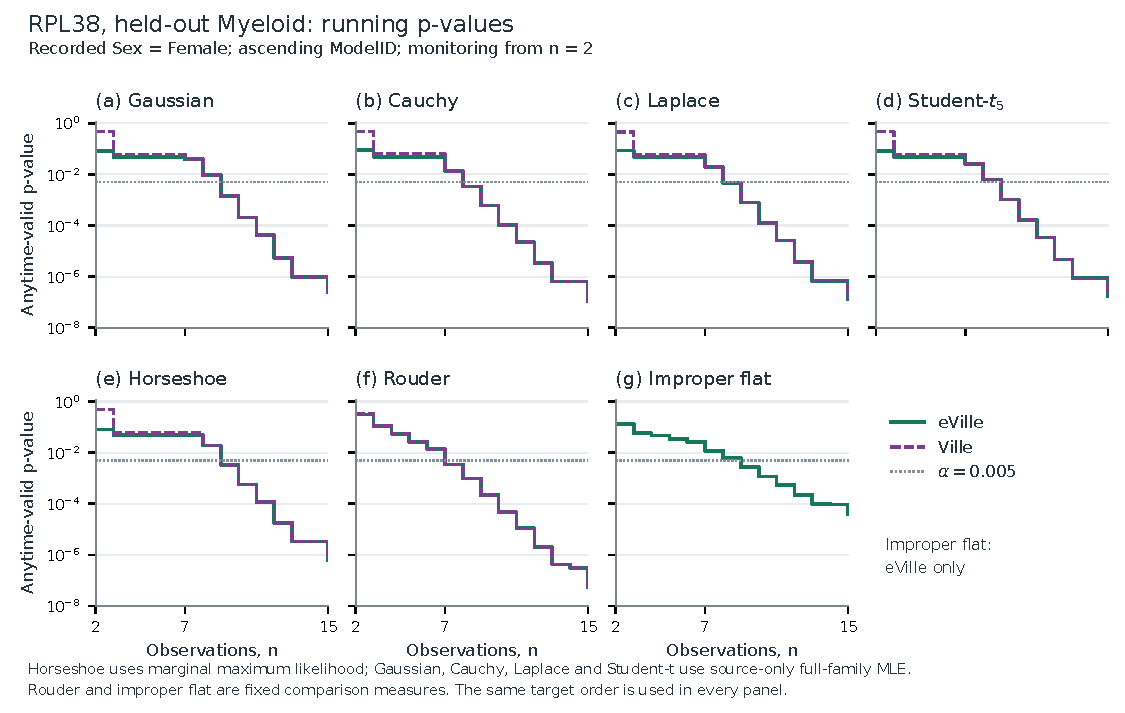
\includegraphics[width=\textwidth]{results/figures/example_running_pvalues.pdf}
\caption{Running anytime-valid $p$-values for the illustrative Myeloid target, monitoring from $n_0=2$ at $\alpha=0.05$ in ascending ModelID order. Priors are fitted using the other eligible lineages only. The Rouder half-Cauchy comparator is fixed, and the improper flat comparator uses genuine Lebesgue measure with eVille calibration only. Horseshoe* uses its stated quantile-fit exception. All paths are evaluated under the same Gaussian working model.}
\label{fig:rpl38-paths}
\end{figure}
